\section{Test Kolmogorov}

Devi utilizzare questa sezione solo se il numero delle \textbf{osservazioni
      totale $n < 30$}.

\subsection{Dati Senza Intervalli}

Devi utilizzare questa sezione solo quando hai dei dati \textbf{Senza
      Intervalli}, devi anche fare attenzione che il \textbf{numero di
      osservazioni totali $n < 30$}!!\\

Operazioni da effettuare:

\begin{enumerate}
      \item Riportare i dati in una tabella in Calc:
            \begin{itemize}
                  \item \textit{Colonna categorie}
                  \item \textit{Colonna frequenze $f_i$}
            \end{itemize}
      \item Calcolare:
            \begin{enumerate}
                  \item $f(i) = f_i / n$: frequenze osservate
                  \item Individuare la distribuzione di probabilità adatta (vedi
                        \ref{stimare-distribuzione})
                  \item $p(i)$: probabilità teorica (vedi \ref{pi})
                  \item $d_i = cumsum(f(i))$: somma cumulativa delle $f(i)$
                  \item $D_i = cumsum(p(i))$: somma cumulativa delle $p(i)$
                  \item $D = |d_i - D_i|$: la differenza assoluta
                  \item $D_{max} = \max(D)$: il massimo valore tra le differenze
                        assolute $D$
            \end{enumerate}
\end{enumerate}

Una volta completati tutti i calcoli, cercare nella tabella di
\textit{Kolmogorov-Smirnov} (vedi \ref{tabella-kolmogorov}) la riga corrispondente al valore delle osservazioni
totali $n$: se il valore $D_{max}$ è sotto il $D_{0,10}$ la distribuzione è
accettata, altrimenti no.

\subsection{Dati Con Intervalli}

Devi utilizzare questa sezione solo quando hai dei dati \textbf{Senza
      Intervalli}, devi anche fare attenzione che il \textbf{numero di
      osservazioni totali $n < 30$}!!\\

\textbf{N.B.}: \textit{non abbiamo trovato esercizi con cui testare questa
      sezione !}\\

Operazioni da effettuare:

\begin{enumerate}
      \item Riportare i dati in una tabella in Calc:
            \begin{itemize}
                  \item \textit{Colonna categorie}: probabilmente devi aggiungerle
                        tu, parti da 0 in poi
                  \item \textit{Colonna intervallo}: del tipo $x_1 - x_2$. Fai
                        sempre attenzione che $x_2 \ge x_1$ !!! In caso li inverti.
                  \item \textit{Colonna frequenze $f_i$}
            \end{itemize}
      \item Aggiungere \textit{Colonna $x_1$} (estremo più piccolo
            dell'intervallo)
      \item Aggiungere \textit{Colonna $x_2$} (estremo più grande dell'intervallo)
      \item Calcolare:
            \begin{enumerate}
                  \item $f(i) = f_i / n$: frequenze osservate
                  \item Individuare la distribuzione di probabilità adatta (vedi
                        \ref{stimare-distribuzione})
                  \item $p(i) = p(x_2) - p(x_1)$: probabilità teorica per ogni
                        intervallo (vedi \ref{pi})
                  \item $d_i = cumsum(f(i))$: somma cumulativa delle $f(i)$
                  \item $D_i = cumsum(p(i))$: somma cumulativa delle $p(i)$
                  \item $D = |d_i - D_i|$: la differenza assoluta
                  \item $D_{max} = \max(D)$: il massimo valore tra le differenze
                        assolute $D$
            \end{enumerate}
\end{enumerate}

Una volta completati tutti i calcoli, cercare nella tabella di
\textit{Kolmogorov-Smirnov} (vedi \ref{tabella-kolmogorov}) la riga corrispondente al valore delle osservazioni
totali $n$: se il valore $D_{max}$ è sotto il $D_{0,10}$ la distribuzione è
accettata, altrimenti no.

\section{Informazioni utili su Formule}

\subsection{Komorov}

\subsubsection{\textit{cumsum}}

Per calcolare $cumsum$ (somma cumulativa) va eseguito il seguente procedimento:
\begin{itemize}
      \item La prima cella resta uguale alla prima cella della colonna di
            riferimento (es. $f(i)$ o $p(i)$)
      \item Dalla seconda cella in poi si blocca la prima cella della somma
            cumulativa (quella calcolata al punto precedente) e si somma fino alla
            cella $i$ di riferimento (vedi Figura \ref{cumsum})
\end{itemize}

\begin{figure}[H]
      \centering
      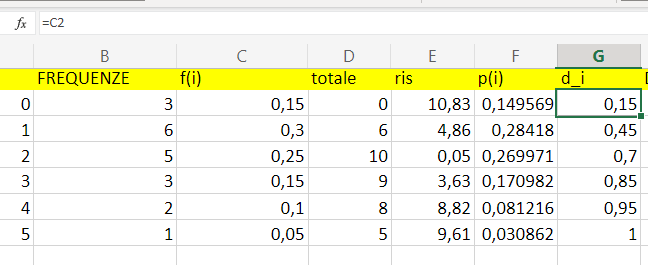
\includegraphics[width=6cm, keepaspectratio]{capitoli/goodnes_of_fit/imgs/cumsum1.png}
      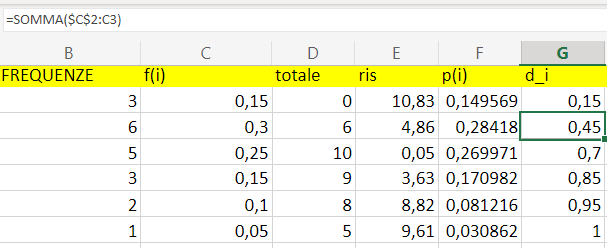
\includegraphics[width=6cm, keepaspectratio]{capitoli/goodnes_of_fit/imgs/cumsum2.png}
      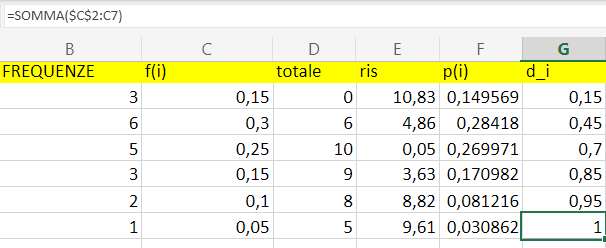
\includegraphics[width=8cm, keepaspectratio]{capitoli/goodnes_of_fit/imgs/cumsum3.png}
      \caption{Esempio di calcolo della funzione $cumsum$}
      \label{cumsum}
\end{figure}